\documentclass[12pt]{article}

% Page geometry
\usepackage[a4paper,margin=1in]{geometry}

% Font and encoding
\usepackage[utf8]{inputenc}
\usepackage[T1]{fontenc}
\usepackage{lmodern}

% Math and physics
\usepackage{amsmath, amssymb, amsfonts}
\usepackage{physics}

% Neural network diagrams
\usepackage{tikz}
\usetikzlibrary{positioning,arrows.meta,calc,shapes,decorations.pathmorphing}
\usepackage{tikz-network}

% Figures and graphics
\usepackage{graphicx}
\usepackage{caption}
\usepackage{subcaption}

% Miscellaneous
\usepackage{hyperref}
\hypersetup{colorlinks=true, linkcolor=blue, urlcolor=blue, citecolor=blue}
\usepackage[parfill]{parskip}

% Custom section numbering: Sections (numbers), Subsections (Roman numerals), Subsubsections (letters)
\renewcommand\thesection{\arabic{section}}
\renewcommand\thesubsection{\Roman{subsection}}
\renewcommand\thesubsubsection{\alph{subsubsection}}

% Ensure numbering is shown for all section levels
\setcounter{secnumdepth}{3}

% Make all section headings smaller
\usepackage{sectsty}
\sectionfont{\large}
\subsectionfont{\normalsize}
\subsubsectionfont{\small}

% Bibliography
\usepackage[backend=bibtex,style=numeric]{biblatex}
\addbibresource{refs.bib}

\usepackage[title]{appendix}

\begin{document}

\begin{titlepage}
	\centering
	\vspace*{2cm}
	{\Huge\bfseries Learned Contour Deformations in Lattice Field Theory\par}
	\vspace{2cm}
	{\Large Ali Shakir\par}
	\vspace{1.5cm}
	\vfill
	
\includegraphics[width=0.2\textwidth]{crest.pdf}\par
	\vspace{0.5cm}
	{\large Supervisor: Dr. Gurtej Kanwar\par}
	\vspace{0.5cm}
	{\large School of Physics and Astronomy\par}
	{\large The University of Edinburgh\par}
	\vspace{1cm}
	{\large \today\par}
\end{titlepage}

\section*{Declaration}

I declare that this work was composed entire by myself, Ali Mehlam Shakir.

Chapter 2 contains a review of the necessary theory around the XY-Model and Markov Chain Monte Carlo (MCMC) simulation.
The relevant derivations are not new work, however implementation of the model simulation using existing approaches was
carried out entirely by myself.

Chapter 3 contains a review of work previously carried out by my supervisor Dr. Gurtej Kanwar, and his colleagues, along with
the details of how we adapt those developments to the specific problem tackled in this work.

The model design and implementation in Chapter 4 is entirely new work carried out by myself with guidance from Dr. Kanwar,
and similarly the results reported in Chapter 5 have not been previously explored in the literature to our knowledge. The
machine learning approaches that we employed are ones that have been circulating in the literature for some time, however
novel modifications were made to adapt them to this particular use case.

\newpage

\section*{Personal Statement}

I spent the early days of the project familiarizing myself with key concepts in lattice field theory, and brushing off my skills coding
in C so that I could first implement a simulation of the XY-Model first using a simple Metropolis-Hastings update and then using the more
sophisticated Wolff cluster update.

Once Dr. Kanwar and I were confident the simulation results were sensible, and that we were able to evaluate key observables of the XY-model
accurately, I began reading about the theory behind contour deformations for reducing noise in the two-point correlator. I also spent a large
portion of time focused on familiarizing myself with PyTorch so that we could begin studying the use of neural networks to produce optimal contour
deformations for the XY-model.

We first began by exploring the use of a one-layer convolutional network to better understand if improving noise on the two-point correlator
via contour deformation would be possible. After confirming a substantial improvement, we moved on to more sophisticated methods.

I then spent the majority of the summer refining the design of model we ultimately sought to use, the U-Net, and making modifications to the architecture
to incorporate a temperature-dependence.

Throughout August I primarily focused on refining figures and writing up this report full-time.

\section*{Acknowledgements}

I would like to thank my supervisor Dr. Kanwar for making this project possible and for his invaluable feedback and guidance
throughout the research and writing phases of the project. I would also like to thank the Higgs Centre for the financial support
offered to me throughout my studies via the Higgs Scholarship.

\newpage

\section*{Abstract}

In this project we explore the use of vertical shift contour deformations to improve noise on the two-point correlation function of the
two-dimensional XY-model.

The XY-model suffers from noisy estimates of the two-point correlator due to sign problems which we find can be alleviated signficantly through
the use of countour deformations whereby the path integral of the system is carried out over a manifold in complexified space. Vertical shift deformations
make up a small subset of possible contour deformations in which only an imaginary offset is added to the single real parameter at each lattice site.

We first explore the feasibility of such a procedure using a 1-layer convolutional neural network to produce a the vertical shifts for each site at fixed temperature,
then move on to the use of a much larger U-Net based architecture to learn the structure of the optimal vertical shift field across a range of temperatures.

We find that substantial improvement can be attained through the use of the U-Net architecture, and study the shape of the shift field as temperature and
distance are varied, as well as produce new plots of the correlation function to illustrate the improvement in estimation of the correlation length.


\newpage

\tableofcontents

\newpage

\section{Introduction}

In this work we are concerned with evaluating two-point correlators of the XY Model in $D=2$. The XY model in two dimensions assigns a two-component unit vector or "spin"
(specified completely by a real angle) to each point on a square lattice with a nearest neighbor interaction proportional to the alignment between spins, and hence is an example of a 
nonlinear $O(2)$ model. The two-point correlator then measures the degree (on average) to which spins at two separate points are aligned.
This model defines the universality class for thin film superfluids (in analogy with superconductivity, superfluidity describes a fluid that flows with zero viscosity), 
and for this reason is of great practical and theoretical significance.

As the lattice size grows large, explicitly computing the path integral for the theory, which would integrating over all possible directions of all spins on the lattice,
quickly becomes intractable, so we turn to Monte Carlo sampling to draw from the distribution governing field configurations by randomly stepping around the domain
of integration in a way that prefers spending more time in areas with large contributions to the integral. Given a set of samples, we can compute the alignment of two
particular spins in each sample and average over all samples to arrive at the correlator.

Kosterlitz and Thouless \cite{KT} showed in 1973 that, despite the Mermin-Wagner theorem forbidding a phase transition due to spontaneous symmetry breaking
in two dimensions, the XY model exhibits a phase transition of infinite order at finite temperature. The phase transition is characterized by a diverging
exponential correlation length, and so the two-point correlation function of the model is of particular interest in simulation. Precise estimates of the KT transition
temperature have previously been made using other observables \cite{Hasenbusch_2005}, however a precise understanding of the correlator is limited by
the tendency of correlation estimates at large separation to suffer from a severe sign problem. Sign problems arise with highly oscillatory observables, for which
estimation becomes noisy when sampling is not also balanced around the center of oscillation.

Past work by Detmold et. al. \cite{Detmold_2021} has demonstrated the feasibility of path integral contour deformations, that is, evaluation
of the path integral over a manifold in complexified space, to alleviate the issue of decaying signal-to-noise in estimates of Wilson loops for lattice $SU(N)$ gauge theory.
Numerical optimization was used to search for optimal manifolds within a subset of possible deformations dubbed vertical shift deformations, where an imaginary offset is added to the
real-valued parameters at each site. Further work \cite{detmold2023signaltonoiseimprovementneuralnetwork} has also demonstrated the ability of sufficiently expressive convolutional neural networks
to determine optimal vertical shift deformations when trained to minimize variance in a particular observable over a set of Monte Carlo samples.

In this work we seek to apply these developments to evaluation of the two-point correlator in the XY model. We first investigate the use of a simple one-layer
convolutional network to evaluate the correlator at fixed temperature and separation, and then move on to a far more expressive U-Net \cite{ronneberger2015unetconvolutionalnetworksbiomedical}
based architecture which additionally implements feature wise linear modulation \cite{perez2017filmvisualreasoninggeneral} to incorporate separation and temperature dependence. In both cases,
a fully-convolutional network (FCN) is applied to an input image inspired \textit{a-priori} by the geometry of the correlator to generate a field of vertical shifts which are applied to
the real-valued angle at each lattice site.

\section{Background}

In this section we provide an overview of the theory around the XY model and the Kosterlitz-Thouless transition before turning to the key concepts in computational
lattice field theory required for simulating the theory and extracting estimates of observables.

\subsection{The XY-Model in 2D}

\subsubsection{The XY Hamiltonian}

The Hamiltonian for the XY model on a square lattice $\Lambda$ with spacing $a$ is as follows:

\begin{equation}
	H[\theta] = -\sum_{\mathbf{r}r\in\Lambda}\sum_{\mu=1,2}\cos(\theta(\mathbf{r}+a\hat{\pmb{\mu}})-\theta(\mathbf{\mathbf{r}}))
\end{equation}

Where we write the two-component vector describing the position of an angle in the lattice as $\mathbf{r}$ and $\hat{\mathbf{\mu}}$ is the unit vector
pointing in the $\mu$-th direction. The cosine simply describes a dot product between two-component unit vectors, which are fully described by one
real-valued angle. It can be seen immediately that the interaction is highly localized --- each spin interacts only with its nearest neighbors. This fact places
the XY model in the regime described by the Mermin-Wagner theorem, which states that continuous symmetries (here $O(2)$ symmetry) cannot
be broken spontaneously at finite temperature in less than three dimensions.

The partition function for the system is then readily written as

\begin{equation} \label{eq:partition}
	\mathcal{Z} = \prod_{\mathbf{r}\in\Lambda}\int_{-\pi}^{\pi}\mathrm{d}\theta(\mathbf{r})\,\exp\left(-\beta H[\theta] \right)
\end{equation}

integrating the Boltzmann factor over all degrees of freedom, i.e. all $L\times L$ sites on a lattice of length $L$. In principle we are concerned with the infinite $L$ regime
however for the purposes of simulation we simply choose $L$ to be large enough to study the long-range correlations of the system. In this work we will use
units in which $k_B=1$ so that $\beta$ may be interchanged simply with $1/T$

In order to make progress with studying the model analytically, it is necessary to go to the continuum limit. Here we follow the derivation shown in
\cite{drouintouchette2022kosterlitzthoulessphasetransitionintroduction}.
We start by considering the regime where the field $\theta$ is slowly varying, so we may expand the cosine to second order:

\begin{equation}
	\cos(\theta(\mathbf{r}+a\hat{\pmb{\mu}})-\theta(\mathbf{\mathbf{r}})) \approx 1 - \frac{1}{2}\left( \theta(\mathbf{r}+a\hat{\pmb{\mu}})-\theta(\mathbf{\mathbf{r}}) \right)^2
\end{equation}

as well as expand the field around $\mathbf{r}$

\begin{equation}
	\theta(\mathbf{r}+a\hat{\pmb{\mu}}) \approx \theta(\mathbf{r}) + a\partial_{\mu}\theta(\mathbf{r})
\end{equation}

Then, bringing out a factor of $a^2$ and carrying out the sum over $\mu$ allows us to take $a \rightarrow 0$ and change the sum over sites for a continuous integral:

\begin{equation}\label{eq:cont_ham}
	\int\mathrm{d}^2 r \, \frac{1}{2}\left( \nabla\theta(\mathbf{r}) \right)^2
\end{equation}

Where we have dropped the infinite constant associated with the zero-th order term in the expansion of cosine.

This form of the Hamiltonian allows for explicit calculation of some observables, particularly the pointwise correlation in the slowly varying (i.e. low temperature) regime.
The continuum form of the Hamiltonian will again be relevant later as we discuss the analytic approach to deforming the path integral.

\subsubsection{Correlation Functions}

The form of the Hamiltonian shown in eq. \ref{eq:cont_ham} can be easily fourier transformed, and the lattice spacing reintroduced:

\begin{equation}
	\int \frac{\mathrm{d}^2 k}{(2\pi)^2} \, \frac{1}{2} k^2 \left|\theta(\mathbf{k})\right|^2 \rightarrow \frac{a^2}{L^2} \sum_{\mathbf{k}} k^2 \left| \theta(\mathbf{k}) \right|
\end{equation}

where, for a real-valued field we uses $\theta^*(\mathbf{k})=\theta(-\mathbf{k})$ and the sum runs over the first Brillouin zone.

Shown in detail in \cite{drouintouchette2022kosterlitzthoulessphasetransitionintroduction}, the field can be decomposed into its real and imaginary parts, so that the
spin-spin correlation

\begin{equation}
	C(\mathbf{r}) = \langle e^{i\theta(\mathbf{r}) - i\theta(\mathbf{0})} \rangle = \frac{1}{\mathcal{Z}} \int \mathcal{D}\theta \, e^{i\theta(\mathbf{r}) - i\theta(\mathbf{0})} e^{-\beta H[\theta]}
\end{equation}

may be evaluated using the standard techniques of gaussian integration.

The correlation function depends only on the magnitude of the separation and takes a power-law form proportional to

\begin{equation}
	g(r) \propto \left(\frac{\pi r}{a}\right)^{-\eta(\beta)}
\end{equation}

illustrating that, in the low temperature regime the system exhibits an infinite correlation length $\xi$, as $\xi$ is defined through (in two dimensions)

\begin{equation}
	g(r) \propto \frac{e^{-r/\xi(\beta)}}{r^{\eta}}
\end{equation}

in the language of statistical field theory, the XY model has a quasi-long-range order at low temperature, and therefore must undergo a phase transition
at finite temperature before reaching the disordered phase. This is the Kosterlitz-Thouless Transition. 

In brief, the particular observable which is thought to jump discontinuously at the KT transition is the helicity modulues $\Upsilon$ which measures the 
response of the lattice (with periodic boundary conditions) to a twisting of the spins along the boundary by an angle $\alpha$. On the lattice, the so-called
Nelson-Kosterlitz jump is smoothed out by finite-size effects, however the drop becomes increasingly sharp as $L$ is increased.

$\Upsilon$ is formally defined through

\begin{equation}
	\Upsilon = -\frac{\partial^2\mathcal{Z}(\alpha)}{\partial\alpha^2}\Big|_{\alpha=0} = \left\langle \sum_{\mathbf{r}\in\Lambda} \cos(\theta(\mathbf{r})-\theta(\mathbf{r}-a\hat{\mathbf{x}}))
	+\left( \sum_{\mathbf{r}\in\Lambda} \sin(\theta(\mathbf{r})-\theta(\mathbf{r}-a\hat{\mathbf{x}})) \right)^2 \right\rangle
\end{equation}

The choice of the $x$ direction here is arbitrary, and if so desired, $\Upsilon$ can be recomputed exchanging $x$ for $y$ to average the two results
and drive noise down further.

Other quantities of diagnostic interest are the squared magnetization per site, which is the square of the generally
nonzero net magnetization per site vector obtained from averaging together all spin vectors on the lattice:

\begin{equation}
	\left\langle \left|\frac{\mathbf{M}}{L^2}\right|^2 \right\rangle = \left\langle \left( \frac{1}{L^2}\sum_{\mathbf{r}\in\Lambda} \cos(\theta(\mathbf{r})) \right)^2 + \left( \frac{1}{L^2}\sum_{\mathbf{r}\in\Lambda} \sin(\theta(\mathbf{r})) \right)^2 \right\rangle
\end{equation}

And the specific heat capacity:

\begin{equation}
	c_V = \frac{\langle H^2 \rangle - \langle H \rangle^2}{L^2 T^2}
\end{equation}

As the hamiltonian $H$ for the XY model is also the total energy associated with a configuration.

Previous work by Hasenbusch et. al. \cite{Hasenbusch_2005} has simulated the model up to very large lattice sizes, utilizing several months of compute
time to study finite-size effects and narrow in estimates of the KT temperature. 

\subsection{Lattice Field Theory}

\subsubsection{Markov Chain Monte Carlo}

The partition function for the XY model on an $L\times L$ square lattice \ref{eq:partition} necessarily involves an integral over all $L\times L$ real variables.
Brute-force evaluation of this integral quickly becomes infeasible as $L$ grows large, therefore we employ random sampling from the distribution to approximate
the integral. Markov Chain Monte Carlo randomly walk around the domain of integration, preferentially moving to areas with large contributions to the integral.

The basic idea is to draw field configurations sequentially $\theta^{(0)} \rightarrow \theta^{(1)} \rightarrow ... \rightarrow \theta^{(t)}$ that will be
distributed according to the Boltzmann measure as $t\rightarrow\infty$. The update that takes $\theta^{(i)}\rightarrow\theta^{(i+1)}$ must satisfy four conditions \cite{hanada2018markovchainmontecarlo}:

\begin{itemize}
	\item The probability of sampling a configuration $\theta^{(t)}$ depends only on the previous configuration $\theta^{(t-1)}$
	\item Any field configuration must be reachable in a finite number of updates
	\item The chain of configurations sampled must be aperiodic
	\item The detailed balance condition: $e^{-\beta H(\theta^{(t)})}\text{Pr}(\theta^{(t)}\rightarrow\theta^{(t')})=e^{-\beta H(\theta^{(t')})}\text{Pr}(\theta^{(t')}\rightarrow\theta^{(t)})$
\end{itemize}

As pointed out in \cite{hanada2018markovchainmontecarlo}, the last of these conditions is perhaps the most nebulous. In brief, if the chain converges to some
distribution asymptotically, it must then be invariant under translation in time, or \textit{stationary}. Enforcing this property gives rise to detailed balance.

In practice we must also account for \textit{thermalization time} $t_0$, that is, if the initial field configuration is very far from the energetic minimum, some number of steps
will be required before the field is consistently fluctuating about equilibrium.

Once a set of field configurations has been gathered, estimating an observable $\mathcal{O}$ that is a function of the field is as simple as computing

\begin{equation}
	\langle \mathcal{O} \rangle = \lim_{t \to \infty} \frac{1}{t-t_0} \sum_{i=t_0}^{t} \mathcal{O}[\theta^{(i)}]
\end{equation}

We may additionally be interested in estimating the noise on our observable, in which case the more sophisticated methods of bootstrap or jackknife resampling
are required. There is also the issue of \textit{autocorrelation time}. We first define the \textit{autocorrelation}, which measures how correlated 
the samples in a sequence are with one another, as:

\begin{equation}
	\rho(t) = \frac{\left\langle \theta^{(i)}\cdot\theta^{(i+t)} \right\rangle}{\sqrt{\mathrm{Var}[\theta^{(i)}]\cdot\mathrm{Var}[\theta^{(i+t)}]}}
	\in [0,\,1]
\end{equation}

Which depends only on the number of iterations or timesteps between when samples are drawn $t$ and not on the absolute step. Without delving too deeply into
the rich field of time series analysis which involves the study of sequences of random variables, we will simply state that the autocorrelation
is expected to decay exponentially with some characteristic time $\tau$.

Autocorrelations mean in practice that we only keep every $n$-th sample with $n$ on the order of $\tau$ to optimize the tradeoff between gaining new information and the computational cost
of saving out field configurations and/or observable values. The presence of correlations between successive data points means that estimates of the mean of those points
will converge to the true value far more slowly.

A common choice of update is the Metropolis-Hastings algorithm, however Metropolis-Hastings is only designed to update one spin on the lattice at a time, therefore
it suffers from critical slowing down near the phase transition. Unlike for quantum field theories, there is a solution to this problem for spin systems in the form
of the Wolff cluster update \cite{PhysRevLett.62.361}.

\subsubsection{The Wolff Cluster Update}

The Wolff update works by, on each iteration, selecting a random spin and forming a cluster of spins which are all flipped at once. The algorithm works as follows,
denoting the spin at site $\mathbf{r}$ by $\mathbf{s}(\mathbf{r})$:

\begin{itemize}
	\item First a random site $\mathbf{r}_0$ is selected along with a randomly oriented plane (a line in the $D=2$ case) with normal vector $\mathbf{\hat{n}}$
	\item The spin is reflected over this plane
	\item Each nearest-neighbour to the spin with location $\mathbf{r}_1$ is added to the cluster with with probability \[
		      1-\exp\{\min[0,2\beta(\mathbf{\hat{n}} \cdot \mathbf{s}(\mathbf{r}_0))(\mathbf{\hat{n}} \cdot \mathbf{s}(\mathbf{r}_1))]\}
	      \]
\end{itemize}

When no neighbors are added to the cluster, cluster formation stops and al. spins are flipped over the chosen plane.

This update can be shown to satisfy the conditions for a Markov Chain. In addition to circumventing the problem of critical slowing down, the Wolff update, particularly
at low temperature, drastically reduces autocorrelation between successive samples. When only a single spin is flipped, successive samples are extremely similar --- on the other hand, when large portions of the lattice are updated, successive samples become decorrelated, and the
system thermalizes faster. Clusters tend to consume much larger portions of the lattice at low temperatures, as is clear from the $\beta$ dependence of probability for 
adding neighbors.

The Wolff update implicitly assumes a nearest-neighbor dot-product interaction, and therefore additionally avoids recalculation of the Hamiltonian at each update step ---
an expensive operation that requires looping over every site in the lattice. As an aside, an update strategy of this kind is applicable to all spin system with spin vectors
lying in any number of dimensions, allowing its use in simulation of the related Heisenberg and Ising models as well.

\subsubsection{Sign Problems}

The two-point correlator is an example of a highly oscillatory observable when the signal becomes weak. In order for the average value of the correlator to approach zero, 
as it should at large separation, individual samples must necessarily be almost evenly distributed around the unit circle in the complex plane (recall that the correlator 
is an exponential of a pure imaginary phase factor). \ref{fig:sign_problem} provides an elementary illustration of the problem for a hypothetical observable that oscillates 
in one dimension.

\begin{figure}[h]
	\centering
	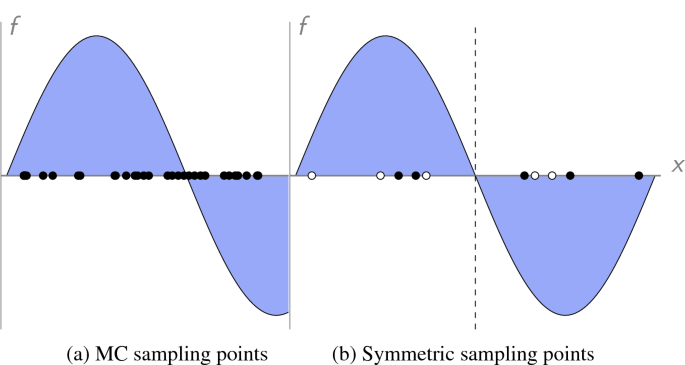
\includegraphics[width=0.6\textwidth]{figures/sign.png}
	\caption{An illustration of a numerical sign problem (courtesy of \cite{10.1007/978-3-030-43465-6_11}) for the case of an observable
	which oscillates on the domain of integration. Small deviations in sampling may result in drastically different estimates
	of the observable mean.}
	\label{fig:sign_problem}
\end{figure}

\section{Methodology}

\subsection{Contour Deformations}

\subsubsection{General Theory}

The essential idea behind deforming the path integral is to evaluate observables along a manifold in complexified space. 

The derivation here is adapted from \cite{Detmold_2021}. Without loss of generality
for some arbitrary real-valued field(s) $\phi$ and an observable $\mathcal{O}$ that is a functional of the field(s), we start with:

\begin{equation} \label{eq:undeformed}
	\langle \mathcal{O} \rangle = \frac{1}{\mathcal{Z}} \int \mathcal{D}\phi \, \mathcal{O}[\phi] \, e^{-\beta H[\phi]}
\end{equation}

And introduce a holomorphic change of variables 

\begin{equation*}
	\phi \rightarrow \tilde{\phi}(\phi)
\end{equation*}

The observable can then be equivalently written as an integral over the manifold in complex space $\mathcal{M}$ 
over which the deformed field $\tilde{\phi}$ varies:

\begin{equation} \label{eq:deformed}
	\frac{1}{\mathcal{Z}} \int \mathcal{D}\tilde{\phi} \, \mathcal{O}(\tilde{\phi}) \, e^{-\beta H[\tilde{\phi}]}
\end{equation}

The integral \ref{eq:deformed} can be performed with respect to the undeformed field by introducing a factor of the complex 
Jacobian $J[\phi] = \det \left( \delta \tilde{\phi} / \delta \phi \right)$

\begin{equation*}
	\int \mathcal{D}\phi \, J[\phi] \, \mathcal{O}[\tilde{\phi}(\phi)] \, e^{-\beta H[\tilde{\phi}(\phi)]}
\end{equation*}

We then reintroduce the undeformed Hamiltonian and push the Jacobian into the exponential to write

\begin{equation} \label{eq:rewrite}
	\int \mathcal{D}\phi \, \mathcal{O}[\tilde{\phi}(\phi)] \, e^{-\beta \left( H[\tilde{\phi}(\phi)] - H[\phi] \right) + \log J[\phi]}\, e^{-\beta H[\phi]} 
	= \int \mathcal{D}\phi \, \mathcal{Q}(\tilde{\phi}(\phi)) \, e^{-\beta H[\phi]} 
\end{equation}

Where we have defined the deformed observable $\mathcal{Q}$ through

\begin{equation}
	 \mathcal{Q}(\tilde{\phi}(\phi)) = \mathcal{O}[\tilde{\phi}(\phi)] \, e^{-\beta \left( H[\tilde{\phi}(\phi)] - H[\phi] \right) + \log J[\phi]}
\end{equation}

So long as the observable $\mathcal{O}$ has an analytic continuation to the manifold $\mathcal{M}$, Cauchy's integral theorem guarantees 
$\langle \mathcal{Q} \rangle = \langle \mathcal{O} \rangle$. The key, of course, is that the variance of the deformed observable need not be the
same. In particular, we can see by writing

\begin{equation} \label{eq:variances}
	\begin{split}
	\mathrm{Var}[\Re \mathcal{O}] = \frac{1}{2} \left\langle \left| \mathcal{O}^2 \right| \right\rangle + \frac{1}{2} \left\langle \mathcal{O}^2 \right\rangle 
	- \mathrm{Re}\left[ \left\langle \mathcal{O} \right\rangle^2 \right] \\ 
	\mathrm{Var}[\Re \mathcal{Q}] = \frac{1}{2} \left\langle \left| \mathcal{Q}^2 \right| \right\rangle + \frac{1}{2} \left\langle \mathcal{Q}^2 \right\rangle 
	- \mathrm{Re}\left[ \left\langle \mathcal{Q} \right\rangle^2 \right]
	\end{split}
\end{equation}

that the first two terms of each equation are not the same, while the final is guaranteed to be the same.

Crucially, as seen in the form of \ref{eq:rewrite}, $\mathcal{Q}$ is being sampled with respect to the original Boltzmann measure $\mathcal{D}\phi\, e^{-\beta H[\phi]}$
rather than attempting sampling with respect to the measure of \ref{eq:deformed}. This means we need not make sense of the complex-valued measure (which no
longer satisfies the conditions to be a probability distribution). In addition we may still employ the same MCMC algorithm to evaluate the deformed observable.

This is of particular importance for spin systems like the XY mode, which, as aforementioned, make use of the much more sophisticated Wolff 
cluster update strategy to drastically reduce thermalization time and autocorrelations.

\subsubsection{Vertical Shifts}

Evidently exploring the full space of potential deformations is infeasibly, and likely unnecessary to achieve significant reduction in observable
variance. Past work by Detmold. et. al \cite{Detmold_2021} has explored restricted spaces of possible deformations, dubbed \textit{vertical shifts} where 
each lattice site acquires an imaginary offset. In the following equations we return to the discretized case, where the field is represented
by $L\times L$ variables $\{\phi_i | i\in{1,2,...,L\times L}\}$.

This family of deformations is only sensible for variables periodic on some interval $[\phi_0,\,\phi_1]$ where the contour may begin and end at any point on the 
lines $\mathrm{Re}(\tilde{\phi}) = \phi_0,\,\phi_1$. A visual depiction is given in \ref{fig:contours}.

\begin{figure}
	\begin{center}
	\tikzset{every picture/.style={line width=0.75pt}} %set default line width to 0.75pt        

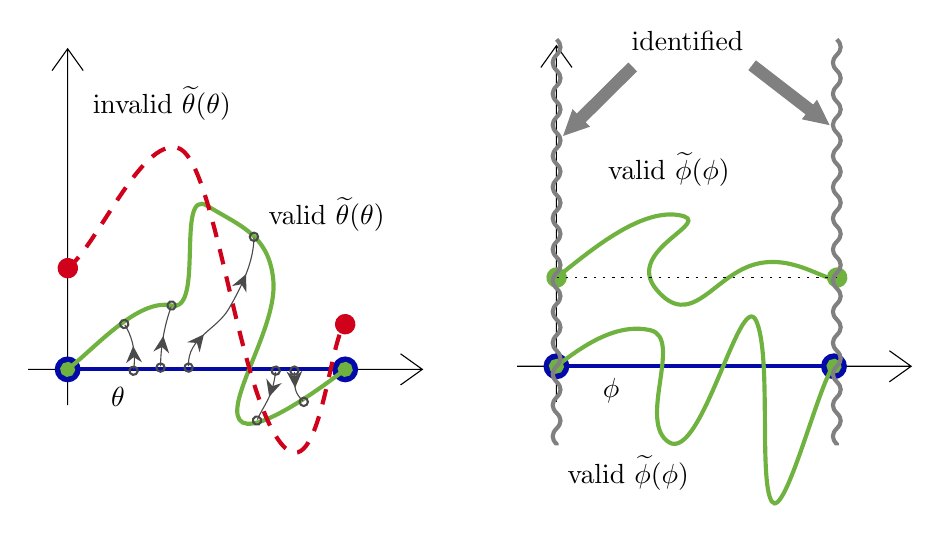
\begin{tikzpicture}[x=0.75pt,y=0.75pt,yscale=-1.5,xscale=1.5]
%uncomment if require: \path (0,310); %set diagram left start at 0, and has height of 310

%Shape: Axis 2D [id:dp25002381159098763] 
\draw  (15,115.58) -- (141.59,115.58)(27.66,12.6) -- (27.66,127.02) (134.59,110.58) -- (141.59,115.58) -- (134.59,120.58) (22.66,19.6) -- (27.66,12.6) -- (32.66,19.6)  ;
%Straight Lines [id:da012448710548571551] 
\draw [color={rgb, 255:red, 3; green, 10; blue, 167 }  ,draw opacity=1 ][line width=1.5]    (27.66,115.58) -- (116.81,115.58) ;
\draw [shift={(116.81,115.58)}, rotate = 0] [color={rgb, 255:red, 3; green, 10; blue, 167 }  ,draw opacity=1 ][fill={rgb, 255:red, 3; green, 10; blue, 167 }  ,fill opacity=1 ][line width=1.5]      (0, 0) circle [x radius= 3.48, y radius= 3.48]   ;
\draw [shift={(27.66,115.58)}, rotate = 0] [color={rgb, 255:red, 3; green, 10; blue, 167 }  ,draw opacity=1 ][fill={rgb, 255:red, 3; green, 10; blue, 167 }  ,fill opacity=1 ][line width=1.5]      (0, 0) circle [x radius= 3.48, y radius= 3.48]   ;
%Curve Lines [id:da22036725062847506] 
\draw [color={rgb, 255:red, 112; green, 178; blue, 63 }  ,draw opacity=1 ][line width=1.5]    (27.66,115.58) .. controls (36.47,108.71) and (50.34,92.65) .. (61.04,95.07) .. controls (71.74,97.5) and (62.19,56.64) .. (72.58,63.08) .. controls (82.97,69.52) and (92.41,72.35) .. (93.73,87.07) .. controls (95.05,101.79) and (78.57,125.26) .. (82.84,131.73) .. controls (87.1,138.21) and (112.47,118.96) .. (116.81,115.58) ;
\draw [shift={(116.81,115.58)}, rotate = 322.05] [color={rgb, 255:red, 112; green, 178; blue, 63 }  ,draw opacity=1 ][fill={rgb, 255:red, 112; green, 178; blue, 63 }  ,fill opacity=1 ][line width=1.5]      (0, 0) circle [x radius= 1.74, y radius= 1.74]   ;
\draw [shift={(27.66,115.58)}, rotate = 322.05] [color={rgb, 255:red, 112; green, 178; blue, 63 }  ,draw opacity=1 ][fill={rgb, 255:red, 112; green, 178; blue, 63 }  ,fill opacity=1 ][line width=1.5]      (0, 0) circle [x radius= 1.74, y radius= 1.74]   ;
%Curve Lines [id:da5448767767433973] 
\draw [color={rgb, 255:red, 208; green, 2; blue, 27 }  ,draw opacity=1 ][line width=1.5]  [dash pattern={on 5.63pt off 4.5pt}]  (27.71,83.07) .. controls (37.31,75.59) and (51.22,41.38) .. (62.97,44.42) .. controls (74.71,47.45) and (81.52,117.49) .. (95.01,137.73) .. controls (108.51,157.97) and (111.6,105.13) .. (116.81,101.07) ;
\draw [shift={(116.81,101.07)}, rotate = 322.05] [color={rgb, 255:red, 208; green, 2; blue, 27 }  ,draw opacity=1 ][fill={rgb, 255:red, 208; green, 2; blue, 27 }  ,fill opacity=1 ][line width=1.5]      (0, 0) circle [x radius= 2.61, y radius= 2.61]   ;
\draw [shift={(27.71,83.07)}, rotate = 322.05] [color={rgb, 255:red, 208; green, 2; blue, 27 }  ,draw opacity=1 ][fill={rgb, 255:red, 208; green, 2; blue, 27 }  ,fill opacity=1 ][line width=1.5]      (0, 0) circle [x radius= 2.61, y radius= 2.61]   ;
%Shape: Axis 2D [id:dp20850113919583269] 
\draw  (172,114.58) -- (298.59,114.58)(184.66,11.6) -- (184.66,126.02) (291.59,109.58) -- (298.59,114.58) -- (291.59,119.58) (179.66,18.6) -- (184.66,11.6) -- (189.66,18.6)  ;
%Straight Lines [id:da009943316285294879] 
\draw [color={rgb, 255:red, 3; green, 10; blue, 167 }  ,draw opacity=1 ][line width=1.5]    (184.66,114.58) -- (273.81,114.58) ;
\draw [shift={(273.81,114.58)}, rotate = 0] [color={rgb, 255:red, 3; green, 10; blue, 167 }  ,draw opacity=1 ][fill={rgb, 255:red, 3; green, 10; blue, 167 }  ,fill opacity=1 ][line width=1.5]      (0, 0) circle [x radius= 3.48, y radius= 3.48]   ;
\draw [shift={(184.66,114.58)}, rotate = 0] [color={rgb, 255:red, 3; green, 10; blue, 167 }  ,draw opacity=1 ][fill={rgb, 255:red, 3; green, 10; blue, 167 }  ,fill opacity=1 ][line width=1.5]      (0, 0) circle [x radius= 3.48, y radius= 3.48]   ;
%Curve Lines [id:da9273036543894462] 
\draw [color={rgb, 255:red, 112; green, 178; blue, 63 }  ,draw opacity=1 ][line width=1.5]    (184.66,114.58) .. controls (193.47,107.71) and (204.13,100.57) .. (214.83,103) .. controls (225.54,105.43) and (210.44,132.56) .. (220.83,139) .. controls (231.23,145.44) and (243.83,89) .. (248.83,100) .. controls (253.83,111) and (249.57,151.53) .. (253.83,158) .. controls (258.1,164.47) and (269.47,117.96) .. (273.81,114.58) ;
\draw [shift={(273.81,114.58)}, rotate = 322.05] [color={rgb, 255:red, 112; green, 178; blue, 63 }  ,draw opacity=1 ][fill={rgb, 255:red, 112; green, 178; blue, 63 }  ,fill opacity=1 ][line width=1.5]      (0, 0) circle [x radius= 1.74, y radius= 1.74]   ;
\draw [shift={(184.66,114.58)}, rotate = 322.05] [color={rgb, 255:red, 112; green, 178; blue, 63 }  ,draw opacity=1 ][fill={rgb, 255:red, 112; green, 178; blue, 63 }  ,fill opacity=1 ][line width=1.5]      (0, 0) circle [x radius= 1.74, y radius= 1.74]   ;
%Curve Lines [id:da4879760234687782] 
\draw [color={rgb, 255:red, 112; green, 178; blue, 63 }  ,draw opacity=1 ][line width=1.5]    (184.71,86.07) .. controls (194.31,78.59) and (210.83,64) .. (223.83,66) .. controls (236.83,68) and (205.83,77) .. (216.83,90) .. controls (227.83,103) and (234.83,86) .. (247.83,82) .. controls (260.83,78) and (271.94,88.33) .. (274.83,86.07) ;
\draw [shift={(274.83,86.07)}, rotate = 322.05] [color={rgb, 255:red, 112; green, 178; blue, 63 }  ,draw opacity=1 ][fill={rgb, 255:red, 112; green, 178; blue, 63 }  ,fill opacity=1 ][line width=1.5]      (0, 0) circle [x radius= 2.61, y radius= 2.61]   ;
\draw [shift={(184.71,86.07)}, rotate = 322.05] [color={rgb, 255:red, 112; green, 178; blue, 63 }  ,draw opacity=1 ][fill={rgb, 255:red, 112; green, 178; blue, 63 }  ,fill opacity=1 ][line width=1.5]      (0, 0) circle [x radius= 2.61, y radius= 2.61]   ;
%Straight Lines [id:da4922067466008355] 
\draw  [dash pattern={on 0.84pt off 2.51pt}]  (184.71,86.07) -- (274.83,86.07) ;
%Straight Lines [id:da19681082381448634] 
\draw [color={rgb, 255:red, 128; green, 128; blue, 128 }  ,draw opacity=1 ][line width=1.5]    (184.71,9.57) .. controls (186.38,11.24) and (186.38,12.9) .. (184.71,14.57) .. controls (183.04,16.24) and (183.04,17.9) .. (184.71,19.57) .. controls (186.38,21.24) and (186.38,22.9) .. (184.71,24.57) .. controls (183.04,26.24) and (183.04,27.9) .. (184.71,29.57) .. controls (186.38,31.24) and (186.38,32.9) .. (184.71,34.57) .. controls (183.04,36.24) and (183.04,37.9) .. (184.71,39.57) .. controls (186.38,41.24) and (186.38,42.9) .. (184.71,44.57) .. controls (183.04,46.24) and (183.04,47.9) .. (184.71,49.57) .. controls (186.38,51.24) and (186.38,52.9) .. (184.71,54.57) .. controls (183.04,56.24) and (183.04,57.9) .. (184.71,59.57) .. controls (186.38,61.24) and (186.38,62.9) .. (184.71,64.57) .. controls (183.04,66.24) and (183.04,67.9) .. (184.71,69.57) .. controls (186.38,71.24) and (186.38,72.9) .. (184.71,74.57) .. controls (183.04,76.24) and (183.04,77.9) .. (184.71,79.57) .. controls (186.38,81.24) and (186.38,82.9) .. (184.71,84.57) .. controls (183.04,86.24) and (183.04,87.9) .. (184.71,89.57) .. controls (186.38,91.24) and (186.38,92.9) .. (184.71,94.57) .. controls (183.04,96.24) and (183.04,97.9) .. (184.71,99.57) .. controls (186.38,101.24) and (186.38,102.9) .. (184.71,104.57) .. controls (183.04,106.24) and (183.04,107.9) .. (184.71,109.57) .. controls (186.38,111.24) and (186.38,112.9) .. (184.71,114.57) .. controls (183.04,116.24) and (183.04,117.9) .. (184.71,119.57) .. controls (186.38,121.24) and (186.38,122.9) .. (184.71,124.57) .. controls (183.04,126.24) and (183.04,127.9) .. (184.71,129.57) .. controls (186.38,131.24) and (186.38,132.9) .. (184.71,134.57) .. controls (183.04,136.24) and (183.04,137.9) .. (184.71,139.57) -- (184.71,140) -- (184.71,140) ;
%Straight Lines [id:da016350095710515156] 
\draw [color={rgb, 255:red, 128; green, 128; blue, 128 }  ,draw opacity=1 ][line width=1.5]    (274.71,9.57) .. controls (276.38,11.24) and (276.38,12.9) .. (274.71,14.57) .. controls (273.04,16.24) and (273.04,17.9) .. (274.71,19.57) .. controls (276.38,21.24) and (276.38,22.9) .. (274.71,24.57) .. controls (273.04,26.24) and (273.04,27.9) .. (274.71,29.57) .. controls (276.38,31.24) and (276.38,32.9) .. (274.71,34.57) .. controls (273.04,36.24) and (273.04,37.9) .. (274.71,39.57) .. controls (276.38,41.24) and (276.38,42.9) .. (274.71,44.57) .. controls (273.04,46.24) and (273.04,47.9) .. (274.71,49.57) .. controls (276.38,51.24) and (276.38,52.9) .. (274.71,54.57) .. controls (273.04,56.24) and (273.04,57.9) .. (274.71,59.57) .. controls (276.38,61.24) and (276.38,62.9) .. (274.71,64.57) .. controls (273.04,66.24) and (273.04,67.9) .. (274.71,69.57) .. controls (276.38,71.24) and (276.38,72.9) .. (274.71,74.57) .. controls (273.04,76.24) and (273.04,77.9) .. (274.71,79.57) .. controls (276.38,81.24) and (276.38,82.9) .. (274.71,84.57) .. controls (273.04,86.24) and (273.04,87.9) .. (274.71,89.57) .. controls (276.38,91.24) and (276.38,92.9) .. (274.71,94.57) .. controls (273.04,96.24) and (273.04,97.9) .. (274.71,99.57) .. controls (276.38,101.24) and (276.38,102.9) .. (274.71,104.57) .. controls (273.04,106.24) and (273.04,107.9) .. (274.71,109.57) .. controls (276.38,111.24) and (276.38,112.9) .. (274.71,114.57) .. controls (273.04,116.24) and (273.04,117.9) .. (274.71,119.57) .. controls (276.38,121.24) and (276.38,122.9) .. (274.71,124.57) .. controls (273.04,126.24) and (273.04,127.9) .. (274.71,129.57) .. controls (276.38,131.24) and (276.38,132.9) .. (274.71,134.57) .. controls (273.04,136.24) and (273.04,137.9) .. (274.71,139.57) -- (274.71,140) -- (274.71,140) ;
%Right Arrow [id:dp761231037087466] 
\draw  [draw opacity=0][fill={rgb, 255:red, 128; green, 128; blue, 128 }  ,fill opacity=1 ] (248.72,16.31) -- (267.13,30.52) -- (268.34,28.94) -- (272.43,37.14) -- (263.47,35.25) -- (264.69,33.68) -- (246.29,19.47) -- cycle ;
%Right Arrow [id:dp13272832472280505] 
\draw  [draw opacity=0][fill={rgb, 255:red, 128; green, 128; blue, 128 }  ,fill opacity=1 ] (210.55,19.84) -- (194.04,36.21) -- (195.45,37.63) -- (186.79,40.6) -- (189.83,31.97) -- (191.24,33.38) -- (207.74,17.01) -- cycle ;
%Curve Lines [id:da07870378678844014] 
\draw [color={rgb, 255:red, 74; green, 74; blue, 74 }  ,draw opacity=1 ]   (48.89,115.58) .. controls (49.73,109) and (47.91,104.23) .. (46.01,101.27) ;
\draw [shift={(45.83,101)}, rotate = 236.31] [color={rgb, 255:red, 74; green, 74; blue, 74 }  ,draw opacity=1 ][line width=0.75]      (0, 0) circle [x radius= 1.34, y radius= 1.34]   ;
\draw [shift={(48.7,108.1)}, rotate = 446.84] [fill={rgb, 255:red, 74; green, 74; blue, 74 }  ,fill opacity=1 ][line width=0.08]  [draw opacity=0] (5.36,-2.57) -- (0,0) -- (5.36,2.57) -- (3.56,0) -- cycle    ;
\draw [shift={(48.83,116)}, rotate = 278.13] [color={rgb, 255:red, 74; green, 74; blue, 74 }  ,draw opacity=1 ][line width=0.75]      (0, 0) circle [x radius= 1.34, y radius= 1.34]   ;
%Curve Lines [id:da7786738388766477] 
\draw [color={rgb, 255:red, 74; green, 74; blue, 74 }  ,draw opacity=1 ]   (57.5,114.64) .. controls (57.54,108.81) and (58.52,102.07) .. (60.93,95.38) ;
\draw [shift={(61.04,95.07)}, rotate = 290.15] [color={rgb, 255:red, 74; green, 74; blue, 74 }  ,draw opacity=1 ][line width=0.75]      (0, 0) circle [x radius= 1.34, y radius= 1.34]   ;
\draw [shift={(58.41,104.84)}, rotate = 457.22] [fill={rgb, 255:red, 74; green, 74; blue, 74 }  ,fill opacity=1 ][line width=0.08]  [draw opacity=0] (5.36,-2.57) -- (0,0) -- (5.36,2.57) -- (3.56,0) -- cycle    ;
\draw [shift={(57.5,115)}, rotate = 270] [color={rgb, 255:red, 74; green, 74; blue, 74 }  ,draw opacity=1 ][line width=0.75]      (0, 0) circle [x radius= 1.34, y radius= 1.34]   ;
%Curve Lines [id:da4539251046582702] 
\draw [color={rgb, 255:red, 74; green, 74; blue, 74 }  ,draw opacity=1 ]   (66.47,114.57) .. controls (66.06,105.35) and (75.56,102.9) .. (79.5,96) .. controls (83.46,89.07) and (87.42,81.16) .. (87.5,73.24) ;
\draw [shift={(87.5,73)}, rotate = 270] [color={rgb, 255:red, 74; green, 74; blue, 74 }  ,draw opacity=1 ][line width=0.75]      (0, 0) circle [x radius= 1.34, y radius= 1.34]   ;
\draw [shift={(71.44,104.33)}, rotate = 489.22] [fill={rgb, 255:red, 74; green, 74; blue, 74 }  ,fill opacity=1 ][line width=0.08]  [draw opacity=0] (5.36,-2.57) -- (0,0) -- (5.36,2.57) -- (3.56,0) -- cycle    ;
\draw [shift={(84.95,84.99)}, rotate = 474.23] [fill={rgb, 255:red, 74; green, 74; blue, 74 }  ,fill opacity=1 ][line width=0.08]  [draw opacity=0] (5.36,-2.57) -- (0,0) -- (5.36,2.57) -- (3.56,0) -- cycle    ;
\draw [shift={(66.5,115)}, rotate = 265.63] [color={rgb, 255:red, 74; green, 74; blue, 74 }  ,draw opacity=1 ][line width=0.75]      (0, 0) circle [x radius= 1.34, y radius= 1.34]   ;
%Curve Lines [id:da11305718845382184] 
\draw [color={rgb, 255:red, 74; green, 74; blue, 74 }  ,draw opacity=1 ]   (94.45,116.4) .. controls (93.43,124.89) and (90.59,126.99) .. (88.62,131.71) ;
\draw [shift={(88.5,132)}, rotate = 111.8] [color={rgb, 255:red, 74; green, 74; blue, 74 }  ,draw opacity=1 ][line width=0.75]      (0, 0) circle [x radius= 1.34, y radius= 1.34]   ;
\draw [shift={(92.4,124.38)}, rotate = 286.65999999999997] [fill={rgb, 255:red, 74; green, 74; blue, 74 }  ,fill opacity=1 ][line width=0.08]  [draw opacity=0] (5.36,-2.57) -- (0,0) -- (5.36,2.57) -- (3.56,0) -- cycle    ;
\draw [shift={(94.5,116)}, rotate = 96.34] [color={rgb, 255:red, 74; green, 74; blue, 74 }  ,draw opacity=1 ][line width=0.75]      (0, 0) circle [x radius= 1.34, y radius= 1.34]   ;
%Curve Lines [id:da9507709065370622] 
\draw [color={rgb, 255:red, 74; green, 74; blue, 74 }  ,draw opacity=1 ]   (100.5,116.35) .. controls (100.5,121.9) and (100.56,123.01) .. (103.28,125.78) ;
\draw [shift={(103.5,126)}, rotate = 45] [color={rgb, 255:red, 74; green, 74; blue, 74 }  ,draw opacity=1 ][line width=0.75]      (0, 0) circle [x radius= 1.34, y radius= 1.34]   ;
\draw [shift={(100.73,121.49)}, rotate = 267.40999999999997] [fill={rgb, 255:red, 74; green, 74; blue, 74 }  ,fill opacity=1 ][line width=0.08]  [draw opacity=0] (5.36,-2.57) -- (0,0) -- (5.36,2.57) -- (3.56,0) -- cycle    ;
\draw [shift={(100.5,116)}, rotate = 90] [color={rgb, 255:red, 74; green, 74; blue, 74 }  ,draw opacity=1 ][line width=0.75]      (0, 0) circle [x radius= 1.34, y radius= 1.34]   ;

% Text Node
\draw (40.76,120.51) node [anchor=north west][inner sep=0.75pt]    {$\theta$};
% Text Node
\draw (34.89,23.86) node [anchor=north west][inner sep=0.75pt]   [align=left] {invalid $\displaystyle \widetilde{\theta }( \theta )$};
% Text Node
\draw (91.37,59.52) node [anchor=north west][inner sep=0.75pt]   [align=left] {valid $\displaystyle \widetilde{\theta }( \theta)$};
% Text Node
\draw (198.76,117.51) node [anchor=north west][inner sep=0.75pt]    {$\phi$};
% Text Node
\draw (200.45,45.03) node [anchor=north west][inner sep=0.75pt]   [align=left] {valid $\displaystyle \widetilde{\phi }( \phi)$};
% Text Node
\draw (187.37,142.52) node [anchor=north west][inner sep=0.75pt]   [align=left] {valid $\displaystyle \widetilde{\phi }( \phi)$};
% Text Node
\draw (208,6) node [anchor=north west][inner sep=0.75pt]   [align=left] {identified};


\end{tikzpicture}
	\end{center}
	\caption{Allowed and disallowed contours for a general variable (courtesy of \cite{Detmold_2021}) $\theta$ and for a periodic variable $\phi$.
	In the case of a periodic variable the slice along the imaginary axis at each end of the interval is identified, 
	so vertical shift deformations are allowed.}
	\label{fig:contours}
\end{figure}

\begin{equation} \label{eq:Jac}
	\tilde{\phi}(\phi) = \phi + if(\phi) \rightarrow J[\phi] = \det\left(\delta_{ij} + i \frac{\partial f_i}{\partial \phi_j} \right)
\end{equation}

In \cite{Detmold_2021}, the cases of a purely upper triangular Jacobian are explored, as well as the use of numerical optimization for the determination of fourier coefficients
for the shift function. In this work we specialize even further to the case where $f$ is simply a position-dependent constant rather than a function of the angles
at each site, so the second term in the determinant of \ref{eq:Jac} drops out and only the identity is left. 

For the remainder of our discussion in this section
we trade $\phi$ back for $\theta$, and represent the position-dependent vertical shifts as $\Delta$. The deformed Hamiltonian now reads 
(using $\langle ij \rangle$ to denote angles $i$ and $j$ are nearest neighbors):

\begin{equation} \label{eq:deformed_ham}
	H[\phi + i \Delta] = -\sum_{\langle ij \rangle} \left(\cos(\theta_i-\theta_j)\cosh(\Delta_i-\Delta_j) -
	i \sin(\theta_i-\theta_j)\sinh(\Delta_i-\Delta_j) \right)
\end{equation}

The deformed Hamiltonian picks up a phase factor that can be tuned to interfere destructively with the phase of the observable of interest. 
Additionally, we see that terms like $\cosh(\Delta_i - \Delta_j)$ which, when entering the exponential, will contribute by reweighting samples. 
Evidently the shift field cannot vary too quickly, as $\cosh$ blows up for large gradients in the shifts. Large gradients will then result in samples being
reweighted by the exponent of a very large negative value, in which case information is lost and the variance will suffer.

\subsubsection{Deforming the Correlator}

As was done to reach \ref{eq:cont_ham}, we can make analytical progress with \ref{eq:deformed_ham} by going to the continuum limit and
expanding the (hyperbolic) trigonometric functions for the case of small variations in the field and the vertical shifts. $\sin$ and $\sinh$ do not
have a second-order term, while $\cos$ and $\cosh$ do, making the analytics particularly straightforward. Keeping only terms quadratic
in the shifts and in the field:

\begin{equation}
	\begin{split}
		cos(\theta_i-\theta_j)\cosh(\Delta_i-\Delta_j) \rightarrow 1 - \frac{1}{2}(\partial_\mu \theta(\mathbf{r}))^2 + \frac{1}{2}(\partial_\mu \Delta(\mathbf{r}))^2 \\
		i \sin(\theta_i-\theta_j)\sinh(\Delta_i-\Delta_j) \rightarrow i(\partial_\mu \theta(\mathbf{r})) \cdot (\partial_\mu \Delta(\mathbf{r}))
	\end{split}
\end{equation}

Again carrying out the sum over $\mu$ and changing the sum for an integral we obtain the continuum deformed Hamiltonian:

\begin{equation}
	H[\phi + i\Delta] = \int \mathrm{d}^2r \left(\frac{1}{2}(\nabla \theta(\mathbf{r}))^2 - \frac{1}{2}(\nabla \Delta(\mathbf{r}))^2 + i \nabla\theta(\mathbf{r}) \cdot \nabla\Delta(\mathbf{r}) \right)
\end{equation}

It is clear that the phase contributed by the deformed Hamiltonian is 

\begin{equation} \label{eq:ham_phase}
	{-\beta\int\mathrm{d}^2r \, \nabla\theta(\mathbf{r})\cdot\nabla\Delta(\mathbf{r})}
\end{equation}

We now require \ref{eq:ham_phase} to interfere with the phase of the two-point correlator of the deformed field, which is 
the exponential of the term

\begin{equation}
	i(\theta(\mathbf{r}) - \theta(\mathbf{0})) -(\Delta(\mathbf{r}) - \Delta(\mathbf{0}))
\end{equation}

So the overall phase of the deformed correlator can be rewritten as (using $\mathbf{x}$ as the integration variable to avoid ambiguity)

\begin{equation}
	\int \mathrm{d}^2x \, \left((\delta(\mathbf{x} - \mathbf{r}) - \delta(\mathbf{x}))\theta(\mathbf{x})-\beta \, \nabla\theta(\mathbf{x})\cdot\nabla\Delta(\mathbf{x})\right)
\end{equation}

In the thermodynamic limit where the boundary lies at infinity, we can integrate the second term by parts at the cost of a sign. Then, setting
the phase to zero produces a Poisson equation with a positive source at $\mathbf{0}$ and a negative source at $\mathbf{r}$. The "charge" of each 
source is scaled by $T=\frac{1}{\beta}$:

\begin{equation} \label{eq:Poisson}
	\nabla^2 \Delta(\mathbf{x}) = -T \left( \delta(\mathbf{x} - \mathbf{r}) - \delta(\mathbf{x}) \right)
\end{equation}

This is a strikingly simple result, however we have only considered the behavior of the deformed Hamiltonian to first order, and when gradients
of the field become large (i.e. high temperature) the approximations that led to this form no longer hold. With this in mind, the main focus of 
this work comes into view --- finding a numerical approach to determining the optimal shift field. In particular, we will investigate the use of 
convolutional neural networks to learn the optimal form of $\Delta$.

\subsection{Machine Learning}

Before delving into our particular use case, we will take a brief detour through the theory of convolutional neural networks for readers
without a strong background in machine learning. A strong understanding of how convolutions and pooling operations are applied to images or stacks of images is crucial
for building the models we use throughout this project.  

To set the stage, a neural network is not much more than a series of linear operations applied to an input, with nonlinear \textit{activation}
functions stitching together successive outputs before applying the next linear operation. Each of those operations ia essentially a tensor of learnable parameters, or \textit{weights} that need
to be tuned, or \textit{trained} to optimize the output.

Training the network involves searching the space of possible \textit{weights} in the model to locate a set of parameters that achieves minimization
of a loss function. Optimization of networks is a constantly evolving field and the methods we employ in this work have a rich
development history. We do not focus heavily on this aspect here, but will include relevant sources as the discussion proceeds. In all cases,
the gradient of the loss with respect to each parameter is required, these gradients being computed through \textit{backpropagation} of gradients from the
final layer of the network to the earliest layers.

\subsubsection{Convolutional Networks}

The vertical shift field itself being an $L \times L$ lattice is particularly conducive to the machinery of fully-convolutional (neural)
networks (FCNs). A fully convolutional network works by accepting an image and performing a series of convolution and pooling operations
to produce another image. 

Discrete convolutions in 2 dimensions utilize a $K\times K$ grid of \textit{learnable} weights, or kernel, which is swept across an input grid, using the weights to take linear combinations of values 
in the input grid as it passes over them and form a new image composed of those combinations. 
In addition to the $K\times K$ weights, an additional additive factor known as a \textit{bias} is also included. In practice, the convolution
may also be applied with nonzero \textit{stride}, in which case the kernel is shifted by more than one site per iteration. This results in a smaller output image.
A simple convolution is illustrated in \ref{fig:conv2d}

Images may also be padded with extra values around the edges before convolution if the image size is not divisible by the kernel size. Padding 
is an important step in our use case to ensure periodicity is preserved by wrapping values from one end over to the other in each dimension.

\begin{figure}[h]
	\begin{center}
	% Fixed data array
\def\inputdata{{
    {0, 4, 1, 0},
    {5, 1, 9, 5},
    {3, 6, 7, 3},
    {0, 4, 1, 0}
}}

\def\kerneldata{{
    {2, 3},
    {1, 6}
}}

\begin{tikzpicture}[scale=0.65]
\definecolor{inputcolor}{RGB}{173,216,230}
\definecolor{kernelcolor}{RGB}{232,95,111}

% Offsets
\def\xoffset{0}
\def\yoffset{0}

% Draw grid and numbers
\foreach \col in {0,...,3} {
    \foreach \row in {0,...,3} {
        % Get value from array (PGF math arrays are zero-based)
        \pgfmathparse{\inputdata[\row][\col]}
        \let\cellvalue\pgfmathresult

        % Check if first row or first column
        \ifnum\row=0
            \def\cellopacity{0.5}
            \def\cellstyle{dashed}
        \else
            \ifnum\col=0
                \def\cellopacity{0.5}
                \def\cellstyle{dashed}
            \else
                \def\cellopacity{1}
                \def\cellstyle{solid}
            \fi
        \fi

        % Draw at shifted position
        \fill[inputcolor,opacity=\cellopacity] (\xoffset+\col,\yoffset-\row) rectangle ++(1,-1);
        \draw[\cellstyle] (\xoffset+\col,\yoffset-\row) rectangle ++(1,-1);

        % Place number centered in shifted position
        \node at (\xoffset+\col+0.5,\yoffset-\row-0.5) {\cellvalue};
    }
}

\foreach \col in {0,...,1} {
    \foreach \row in {0,...,1} {
        % Get value from array (PGF math arrays are zero-based)
        \pgfmathparse{\kerneldata[\row][\col]}
        \let\cellvalue\pgfmathresult

        % Draw at shifted position
        \fill[kernelcolor] (4.5+\col,-1-\row) rectangle ++(1,-1);
        \draw (4.5+\col,-1-\row) rectangle ++(1,-1);

        % Place number centered in shifted position
        \node at (4.5+\col+0.5,-1-\row-0.5) {\cellvalue};
    }
}

\draw[opacity=0.5,thick] (2,0) -- (6.5,-1);
\draw[opacity=0.5,thick] (0,-2) -- (4.5,-3);

\definecolor{outputcolor}{RGB}{144,238,144}

\foreach \col in {0,...,2} {
    \foreach \row in {0,...,2} {
        \fill[outputcolor] (7.5+\col,-0.5-\row) rectangle ++(1,-1);
        \draw (7.5+\col,-0.5-\row) rectangle ++(1,-1);
        % Add number 23 in the first square
        \ifnum\col=0
            \ifnum\row=0
            \node at (7.5+0.5,-0.5-0.5) {23};
            \fi
        \fi
        }
    }

    \draw[->,thick] (6.5,-2) -- (8,-1.2);

    % Draw a second input grid to the right
    \foreach \col in {0,...,3} {
        \foreach \row in {0,...,3} {
            \pgfmathparse{\inputdata[\row][\col]}
            \let\cellvalue\pgfmathresult

            % Check if first row or first column
            \ifnum\row=0
                \def\cellopacity{0.5}
                \def\cellstyle{dashed}
            \else
                \ifnum\col=0
                    \def\cellopacity{0.5}
                    \def\cellstyle{dashed}
                \else
                    \def\cellopacity{1}
                    \def\cellstyle{solid}
                \fi
            \fi

            \fill[inputcolor,opacity=\cellopacity] (12+\col,\yoffset-\row) rectangle ++(1,-1);
            \draw[\cellstyle] (12+\col,\yoffset-\row) rectangle ++(1,-1);
            \node at (12+\col+0.5,\yoffset-\row-0.5) {\cellvalue};
        }
    }

    % Draw a second kernel grid to the right
    \foreach \col in {0,...,1} {
        \foreach \row in {0,...,1} {
            \pgfmathparse{\kerneldata[\row][\col]}
            \let\cellvalue\pgfmathresult
            \fill[kernelcolor] (16.5+\col,-1-\row) rectangle ++(1,-1);
            \draw (16.5+\col,-1-\row) rectangle ++(1,-1);
            \node at (16.5+\col+0.5,-1-\row-0.5) {\cellvalue};
        }
    }

    \draw[opacity=0.5,thick] (15,0) -- (18.5,-1);
    \draw[opacity=0.5,thick] (13,-2) -- (16.5,-3);

    % Draw a second output grid to the right
    \foreach \col in {0,...,2} {
        \foreach \row in {0,...,2} {
            \fill[outputcolor] (19.5+\col,-0.5-\row) rectangle ++(1,-1);
            \draw (19.5+\col,-0.5-\row) rectangle ++(1,-1);
            % Add number 66 in the second square
            \ifnum\col=1
                \ifnum\row=0
                \node at (19.5+1+0.5,-0.5-0.5) {66};
                \fi
            \fi
        }
    }

    \draw[->,thick] (18.5,-2) -- (21,-1.2);
    % Labels under grids
    \node at (2,-5) {input};
    \node at (5.5,-4) {kernel};
    \node at (8.5,-4) {output};

    \node at (14,-5) {input};
    \node at (17.5,-4) {kernel};
    \node at (20.5,-4) {output};

\end{tikzpicture}
	% % Fixed data array

\def\inputdata{{
    {2, 3},
    {1, 6}
}}

\def\kerneldata{{
    {5, 2},
    {3, 1}
}}

\begin{tikzpicture}[scale=0.65]
\definecolor{inputcolor}{RGB}{173,216,230}
\definecolor{kernelcolor}{RGB}{232,95,111}

% Offsets
\def\xoffset{0}
\def\yoffset{0}

% Draw grid and numbers
\foreach \col in {0,...,1} {
    \foreach \row in {0,...,1} {
        % Get value from array (PGF math arrays are zero-based)
        \pgfmathparse{\inputdata[\row][\col]}
        \let\cellvalue\pgfmathresult

        % Draw at shifted position
        \fill[inputcolor] (\xoffset+\col,\yoffset-\row) rectangle ++(1,-1);
        \draw (\xoffset+\col,\yoffset-\row) rectangle ++(1,-1);

        % Place number centered in shifted position
        \node at (\xoffset+\col+0.5,\yoffset-\row-0.5) {\cellvalue};
    }
}
% Draw kernel grid to the right of input grid
\def\kernelxoffset{3} % Shift right by 3 units (2 for input grid + 1 gap)
\def\kernelyoffset{-0.5}

\foreach \col in {0,...,1} {
    \foreach \row in {0,...,1} {
        \pgfmathparse{\kerneldata[\row][\col]}
        \let\cellvalue\pgfmathresult

        \fill[kernelcolor] (\kernelxoffset+\col,\kernelyoffset-\row) rectangle ++(1,-1);
        \draw[thick,black] (\kernelxoffset+\col,\kernelyoffset-\row) rectangle ++(1,-1);

        \node at (\kernelxoffset+\col+0.5,\kernelyoffset-\row-0.5) {\cellvalue};
    }
}

\draw[opacity=0.5,thick] (1,0) -- (5,-0.5);
\draw[opacity=0.5,thick] (0,-1) -- (3,-2.5);

% Define output grid color
\definecolor{outputcolor}{RGB}{144,238,144}

% Output grid offset (to the right of kernel grid)
\def\outputxoffset{6} % 2 for input + 1 gap + 2 for kernel + 1 gap
\def\outputyoffset{0}

% Output grid values (3x3, only top-left 2x2 filled)
\def\outputdata{{
    {10, 4, ""},
    {6, 2, ""},
    {"", "", ""}
}}

% Draw output grid
\foreach \col in {0,...,2} {
    \foreach \row in {0,...,2} {
        \pgfmathparse{\outputdata[\row][\col]}
        \let\cellvalue\pgfmathresult

        \fill[outputcolor] (\outputxoffset+\col,\outputyoffset-\row) rectangle ++(1,-1);
        \draw[thick,black] (\outputxoffset+\col,\outputyoffset-\row) rectangle ++(1,-1);

        % Only show non-empty values
        \ifx\cellvalue\empty
            % Do nothing
        \else
            \node at (\outputxoffset+\col+0.5,\outputyoffset-\row-0.5) {\cellvalue};
        \fi
    }
}

\draw[opacity=0.5,thick] (6,0) -- (3,-0.5);
\draw[opacity=0.5,thick] (8,-2) -- (5,-2.5);

% Shift for second set of grids
\def\secondshift{10}

% Draw second input grid
\foreach \col in {0,...,1} {
    \foreach \row in {0,...,1} {
        \pgfmathparse{\inputdata[\row][\col]}
        \let\cellvalue\pgfmathresult

        \fill[inputcolor] (\secondshift+\xoffset+\col,\yoffset-\row) rectangle ++(1,-1);
        \draw (\secondshift+\xoffset+\col,\yoffset-\row) rectangle ++(1,-1);

        \node at (\secondshift+\xoffset+\col+0.5,\yoffset-\row-0.5) {\cellvalue};
    }
}

% Draw second kernel grid
\foreach \col in {0,...,1} {
    \foreach \row in {0,...,1} {
        \pgfmathparse{\kerneldata[\row][\col]}
        \let\cellvalue\pgfmathresult

        \fill[kernelcolor] (\secondshift+\kernelxoffset+\col,\kernelyoffset-\row) rectangle ++(1,-1);
        \draw[thick,black] (\secondshift+\kernelxoffset+\col,\kernelyoffset-\row) rectangle ++(1,-1);

        \node at (\secondshift+\kernelxoffset+\col+0.5,\kernelyoffset-\row-0.5) {\cellvalue};
    }
}

\draw[opacity=0.5,thick] (\secondshift+2,0) -- (\secondshift+5,-0.5);
\draw[opacity=0.5,thick] (\secondshift+1,-1) -- (\secondshift+3,-2.5);
% Draw second output grid
% Top right 2x2 subgrid: positions (0,1), (0,2), (1,1), (1,2)
\def\secondoutputdata{{
    {"", 15, 6},
    {"", 9, 3},
    {"", "", ""}
}}

\foreach \col in {0,...,2} {
    \foreach \row in {0,...,2} {
        \pgfmathparse{\secondoutputdata[\row][\col]}
        \let\cellvalue\pgfmathresult

        \fill[outputcolor] (\secondshift+\outputxoffset+\col,\outputyoffset-\row) rectangle ++(1,-1);
        \draw[thick,black] (\secondshift+\outputxoffset+\col,\outputyoffset-\row) rectangle ++(1,-1);

        \ifx\cellvalue\empty
        \else
            \node at (\secondshift+\outputxoffset+\col+0.5,\outputyoffset-\row-0.5) {\cellvalue};
        \fi
    }
}

\draw[opacity=0.5,thick] (\secondshift+7,0) -- (\secondshift+3,-0.5);
\draw[opacity=0.5,thick] (\secondshift+9,-2) -- (\secondshift+5,-2.5);

% Labels for first set
\node[below=6pt] at (1,-2) {input};
\node[below=6pt] at (4,-2.5) {kernel};
\node[below=6pt] at (7,-3) {output};

% Labels for second set
\node[below=6pt] at (\secondshift+1,-2) {input};
\node[below=6pt] at (\secondshift+4,-2.5) {kernel};
\node[below=6pt] at (\secondshift+7,-3) {output};

\end{tikzpicture}
	\end{center}
	\caption{How a 2x2 convolution kernel sweeps over a 3x3 input grid with periodic paddingto produce a new 3x3 grid. The first two iterations are shown.
	Notice the output grid is 3x3, since the kernel can be translated to the right (and down) 3 times before reaching the edge of the input.
	A stride of 2 for example would produce a 2x2 output}
	\label{fig:conv2d}
\end{figure}

Convolution can be used to increase the size of an input as well, through an operation called \textit{transpose convolution} wherein the kernel of weights
moves across one site at a time, magnifying it to a $K \times K$ grid. All of the resultant grids are then lined up according to the position they 
multiplied in the input layer, and overlapping values are summed. A simple transpose convolution is illustrated in \ref{fig:transconv2d}

\begin{figure}[h]
	\begin{center}
	% Fixed data array

\def\inputdata{{
    {2, 3},
    {1, 6}
}}

\def\kerneldata{{
    {5, 2},
    {3, 1}
}}

\begin{tikzpicture}[scale=0.65]
\definecolor{inputcolor}{RGB}{173,216,230}
\definecolor{kernelcolor}{RGB}{232,95,111}

% Offsets
\def\xoffset{0}
\def\yoffset{0}

% Draw grid and numbers
\foreach \col in {0,...,1} {
    \foreach \row in {0,...,1} {
        % Get value from array (PGF math arrays are zero-based)
        \pgfmathparse{\inputdata[\row][\col]}
        \let\cellvalue\pgfmathresult

        % Draw at shifted position
        \fill[inputcolor] (\xoffset+\col,\yoffset-\row) rectangle ++(1,-1);
        \draw (\xoffset+\col,\yoffset-\row) rectangle ++(1,-1);

        % Place number centered in shifted position
        \node at (\xoffset+\col+0.5,\yoffset-\row-0.5) {\cellvalue};
    }
}
% Draw kernel grid to the right of input grid
\def\kernelxoffset{3} % Shift right by 3 units (2 for input grid + 1 gap)
\def\kernelyoffset{-0.5}

\foreach \col in {0,...,1} {
    \foreach \row in {0,...,1} {
        \pgfmathparse{\kerneldata[\row][\col]}
        \let\cellvalue\pgfmathresult

        \fill[kernelcolor] (\kernelxoffset+\col,\kernelyoffset-\row) rectangle ++(1,-1);
        \draw[thick,black] (\kernelxoffset+\col,\kernelyoffset-\row) rectangle ++(1,-1);

        \node at (\kernelxoffset+\col+0.5,\kernelyoffset-\row-0.5) {\cellvalue};
    }
}

\draw[opacity=0.5,thick] (1,0) -- (5,-0.5);
\draw[opacity=0.5,thick] (0,-1) -- (3,-2.5);

% Define output grid color
\definecolor{outputcolor}{RGB}{144,238,144}

% Output grid offset (to the right of kernel grid)
\def\outputxoffset{6} % 2 for input + 1 gap + 2 for kernel + 1 gap
\def\outputyoffset{0}

% Output grid values (3x3, only top-left 2x2 filled)
\def\outputdata{{
    {10, 4, ""},
    {6, 2, ""},
    {"", "", ""}
}}

% Draw output grid
\foreach \col in {0,...,2} {
    \foreach \row in {0,...,2} {
        \pgfmathparse{\outputdata[\row][\col]}
        \let\cellvalue\pgfmathresult

        \fill[outputcolor] (\outputxoffset+\col,\outputyoffset-\row) rectangle ++(1,-1);
        \draw[thick,black] (\outputxoffset+\col,\outputyoffset-\row) rectangle ++(1,-1);

        % Only show non-empty values
        \ifx\cellvalue\empty
            % Do nothing
        \else
            \node at (\outputxoffset+\col+0.5,\outputyoffset-\row-0.5) {\cellvalue};
        \fi
    }
}

\draw[opacity=0.5,thick] (6,0) -- (3,-0.5);
\draw[opacity=0.5,thick] (8,-2) -- (5,-2.5);

% Shift for second set of grids
\def\secondshift{10}

% Draw second input grid
\foreach \col in {0,...,1} {
    \foreach \row in {0,...,1} {
        \pgfmathparse{\inputdata[\row][\col]}
        \let\cellvalue\pgfmathresult

        \fill[inputcolor] (\secondshift+\xoffset+\col,\yoffset-\row) rectangle ++(1,-1);
        \draw (\secondshift+\xoffset+\col,\yoffset-\row) rectangle ++(1,-1);

        \node at (\secondshift+\xoffset+\col+0.5,\yoffset-\row-0.5) {\cellvalue};
    }
}

% Draw second kernel grid
\foreach \col in {0,...,1} {
    \foreach \row in {0,...,1} {
        \pgfmathparse{\kerneldata[\row][\col]}
        \let\cellvalue\pgfmathresult

        \fill[kernelcolor] (\secondshift+\kernelxoffset+\col,\kernelyoffset-\row) rectangle ++(1,-1);
        \draw[thick,black] (\secondshift+\kernelxoffset+\col,\kernelyoffset-\row) rectangle ++(1,-1);

        \node at (\secondshift+\kernelxoffset+\col+0.5,\kernelyoffset-\row-0.5) {\cellvalue};
    }
}

\draw[opacity=0.5,thick] (\secondshift+2,0) -- (\secondshift+5,-0.5);
\draw[opacity=0.5,thick] (\secondshift+1,-1) -- (\secondshift+3,-2.5);
% Draw second output grid
% Top right 2x2 subgrid: positions (0,1), (0,2), (1,1), (1,2)
\def\secondoutputdata{{
    {"", 15, 6},
    {"", 9, 3},
    {"", "", ""}
}}

\foreach \col in {0,...,2} {
    \foreach \row in {0,...,2} {
        \pgfmathparse{\secondoutputdata[\row][\col]}
        \let\cellvalue\pgfmathresult

        \fill[outputcolor] (\secondshift+\outputxoffset+\col,\outputyoffset-\row) rectangle ++(1,-1);
        \draw[thick,black] (\secondshift+\outputxoffset+\col,\outputyoffset-\row) rectangle ++(1,-1);

        \ifx\cellvalue\empty
        \else
            \node at (\secondshift+\outputxoffset+\col+0.5,\outputyoffset-\row-0.5) {\cellvalue};
        \fi
    }
}

\draw[opacity=0.5,thick] (\secondshift+7,0) -- (\secondshift+3,-0.5);
\draw[opacity=0.5,thick] (\secondshift+9,-2) -- (\secondshift+5,-2.5);

% Labels for first set
\node[below=6pt] at (1,-2) {input};
\node[below=6pt] at (4,-2.5) {kernel};
\node[below=6pt] at (7,-3) {output};

% Labels for second set
\node[below=6pt] at (\secondshift+1,-2) {input};
\node[below=6pt] at (\secondshift+4,-2.5) {kernel};
\node[below=6pt] at (\secondshift+7,-3) {output};

\end{tikzpicture}
	\end{center}
	\caption{How the transpose operation works by magnifying each site of the input image. Notice that the next iteration shown 
	on the right will overlap the values 4 and 2 from the first iteration. After all iterations are performed, the resultant
	grids are summed together (with the blank spaces being zero)}
	\label{fig:transconv2d}
\end{figure}

We may also desire the input layer at an intermediate convolution to have more than one layer, or \textit{channel}, as well as to produce an output image also
with multiple channels. As an example, consider a typical RGB image, which necessarily has 3 channels describing the amount of each color present in each pixel.
We may think of the stack of three images as a 3-dimensional object, which is now swept over by a kernel of size $3\times K\times K$. Alternatively, this can be thought of
as sweeping a kernel over each channel and adding together the results from each channel at each iteration to "collapse" the channels to a single channel. If we then
want the output image to have $N$ channels, we'll require $N$ independent $3\times K\times K$ kernels, each producing one of the $N$ output channels.

Finally, pooling operations also sweep a kernel across the input with some stride and padding, however rather than multiplying values in the input
they simply perform an operation such as averaging the values overlapped by the kernel, taking the maximum or minimum, or some other simple arithmetic operation. 
No learnable parameters are involved which must be optimized. Pooling operations are typically implemented with a stride that is equal to the size of the kernel so that the size of the input image is
decreased significantly, as the goal is the compress the input information into a smaller amount of meaningful data.

We can form highly expressive networks by chaining the aforementioned operations together with nonlinear operations, or\textit{activation functions} in between applied
to each pixel/site in the layer outputted by the previous convolution.

This is exactly what we will do in creating the U-Net architecture described later in this section. In the past, the primary use of FCNs has been for the task 
of \textit{image segmentation}, which involves detecting the outlines of objects in an image. The input in that case is the image itself, and the output
a usually black-and-white image depicting the outlines of various objects. In our case the input image is a single channel mask inspired \textit{a priori}
by the geometry of the correlator.

\subsubsection{Multilayer Perceptrons}

We will also require the use of \textit{Multilayer Perceptrons} (MLPs). These objects are designed to operate on scalar or vector inputs
rather than images, and are often used in conjunction with convolutional networks to produce scalar outputs for regression or classification tasks.

The MLP is most simply thought of as a form of nonlinear regression. An input vector $\mathbf{x}$ with $n$ components passes through a linear
transformation $\mathbf{A}:\mathbb{R}^n\to \mathbb{R}^m$ to produce a vector with $m$ components, with a single learnable \textit{bias} also added to all components. Each component passes through a nonlinear function $f$ 
before the processes repeats again some number of times. Each linear transformation is a matrix of learnable weights. 

We can represent these networks with flowchart-like diagrams, where intermediate layes are represented by a set of nodes for each component and lines between nodes
indicate a learnable weight. An example of such a diagram appears in \ref{fig:unet}.

\subsubsection{The Input Mask}

As we saw in \ref{eq:Poisson}, the optimal vertical shift deformation for the two-point correlator takes the form of a source at the origin and
a sink at the point of interest. In the continuum limit and with a small gradients approximation, we found the shift field that cancels the phase of
the correlator to take the same form as the electric potential due to two point charges in two dimensions. 

While we expect that the more sophisticated neural network architecture should be able to account for higher-order effects that our approximation drops, 
the general process for producing the shift field should be by "smearing out" opposite-sign point sources at the origin and second point. \ref{fig:mask_to_shift} 
demonstrates this idea assuming the model were to learn simply to solve the Poisson equation of \ref{eq:Poisson}. 

\begin{figure}[h]
	\centering
	\begin{minipage}{0.3\textwidth}
		\centering
		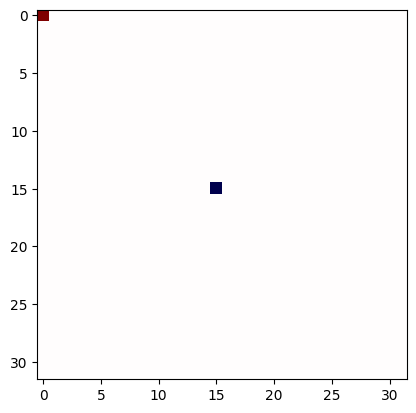
\includegraphics[width=\textwidth]{figures/unsmeared.png}
		\caption*{Input mask}
	\end{minipage}
	\hspace{0.05\textwidth}
	\begin{minipage}{0.1\textwidth}
		\centering
		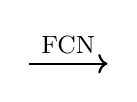
\begin{tikzpicture}[scale=1]
			\draw[->, thick] (0,0.5) -- (1,0.5);
			\node[above] at (0.5,0.5) {\small FCN};
		\end{tikzpicture}
	\end{minipage}
	\hspace{0.05\textwidth}
	\begin{minipage}{0.3\textwidth}
		\centering
		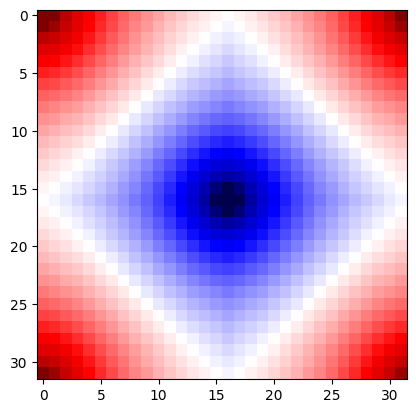
\includegraphics[width=\textwidth]{figures/smeared.png}
		\caption*{Shift field}
	\end{minipage}
	\caption{The input mask (left) with point sources at $(0,0)$ and $(16,16)$ on a $32\times 32$ lattice passes through a convolutional network. 
	to produce a shift field which is "smeared out" across the entire lattice.}
	\label{fig:mask_to_shift}
\end{figure}

In our implementation, discussed in the next section, we will handle generation of the mask internally, so that the network is only required to
take a coordinate $(x,\,y)$ on the lattice as the input. 

\subsubsection{1-Layer Network and Loss Function}

As a springboard for further investigation, we began by using a single convolution applied to the input mask. With only one convolution, the network
only has $K\times K$ parameters, meaning the training routine to optimize these parameters is quick, as is generating the shift masks. The limited
expressivity of such a network means that we cannot expect it to generalize well to arbitrary separation and temperature.

With one convolutional layer there is also the fact that the point sources on the input mask can only be smeared out as far as $K$ from their position.
For this reason we might expect the 1-layer network to work best when the "true" shift field is highly localized around the source and sink. Another way
of looking at this is using the analogy to electrostatics --- the electric field due to two point sources that are sufficiently far apart will mimic
the field due to only one of the charges when in the vicinity of that charge. 

Now is also a good time to discuss the basic single separation, single temperature loss function that will later become a component of the
generalized loss used for training a more sophisticated model. 

Inspired by the form of the variance for the deformed observable \ref{eq:variances}, we optimize for the variance of the real part of the 
deformed correlator, writing the loss function for the network as 

\begin{equation} \label{eq:loss}
	\mathcal{L} = \left\langle \left( \mathrm{Re}\, \mathcal{Q} \right)^2 \right\rangle
\end{equation}

We could also use the imaginary part, but the real part is inspired by the undeformed observable:

\begin{equation*}
	e^{i\theta(\mathbf{r})-i\theta(\mathbf{0})} = \cos\left(\theta(\mathbf{r}) - \theta(\mathbf{0})\right) + i\sin\left(\theta(\mathbf{r}) - \theta(\mathbf{0})\right)
\end{equation*}

The $O(2)$ symmetry of the model mandates that the second term average to zero, in fact it will be symmetrically distributed around zero.
As we will see later when discussing results, minimizing the square of the real part of the deformed observable will have the effect of "squeezing" the distribution of the real part
as much as possible via vertical shift deformation, while of course the mean is preserved by Cauchy's theorem.

\subsubsection{The U-Net, FiLM, and Generalized Loss}

In order to build a network that is sufficiently expressive for generalizing to arbitrary temperature and separation, we turn to the 
U-Net architecture, originally proposed in \cite{ronneberger2015unetconvolutionalnetworksbiomedical}, with some adjustments.

The U-Net was originally developed for biomedical image segmentation, to identify the the structures formed by neurons in 
2D scans from electron microscopes. The original U-Net consists of three basic steps:

\begin{itemize}
	\item The \textit{encoder}: Each encoder level consists of a convolution to double the number of channels followed
	by a SiLU activation \ref{fig:silu}
	
	Feature-wise linear modulation (FiLM), described further below, is then applied
	across the channels before another convolution preserving the number of channels with a SiLU is performed.
	
	Max pooling is then applied to reduce each dimension of the input by a factor of two before the process is repeated.

	\item The \textit{decoder} step: Each decoder level first performs a transpose convolution to double each dimension and halve 
	the number of channels.
	Then, a convolution halves the number of channels again (to offset doubling by the skip connection) before another convolution. The process then repeats

	\item \textit{Skip connections} The skip connections grab the final stage channels of each encoder level and carry them over
	to be appended to the corresponding decoder level, doubling the number of channels in the first stage of that level.

	The idea behind the skip connection is that it allows the network to preserve long-range/large-scale features that are identified
	in the larger images during encoding and carry that information over to decoding. 
\end{itemize}

\begin{figure}
	\begin{center}
	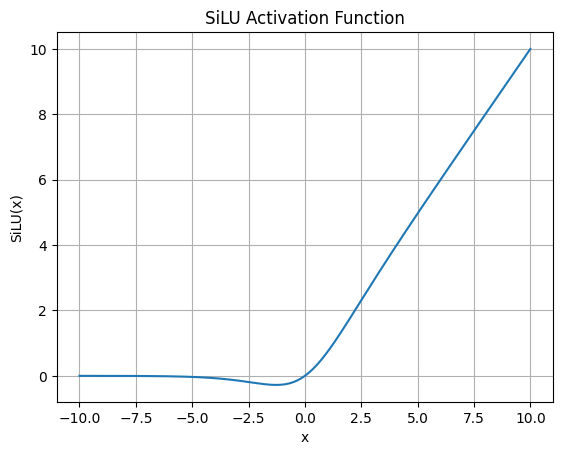
\includegraphics[width=0.6\textwidth]{figures/SiLU.png}
	\end{center}
	\caption{SiLU activation function}
	\label{fig:silu}
\end{figure}

The general shape and description of the operations involved in the U-Net is shown in \ref{fig:unet}. The only unfamiliar operation here
is FiLM, which we will take a brief detour to describe next.

The original implementation of the U-Net required only these three steps. Because we have a scalar input (temperature) in addition to the mask, 
we need a way to feed that information into the encoder steps effectively. The work of \cite{perez2017filmvisualreasoninggeneral} provided inspiration
for how to do this effectively. The implementation of Perez et. al. is significantly more involved than what we require, but the basic idea is easily
adaptable to any scenario where we might seek to condition a convolutional network on information that is not conducive to an image-like representation.

If at some stage of the network, in our case right after the first convolution of each encoder step, we have an image with $C$ channels, we 

\begin{itemize}
	\item treat each channel as an element of a $C$ component vector $\gamma_i$ with $i\in[1,2,...,C]$
	\item We then use an auxilliary network, in our case the MLP shown in the bottom part of \ref{fig:unet}
	to generate $C$ component vectors $\alpha_i$ and $\beta_i$ which are \textit{scaling} and \textit{bias} factors, respectively
	\item Pass the channels $\alpha_i \cdot \gamma_i + \beta_i$ into the next convolution
\end{itemize} 

\begin{figure}
	\begin{center}
	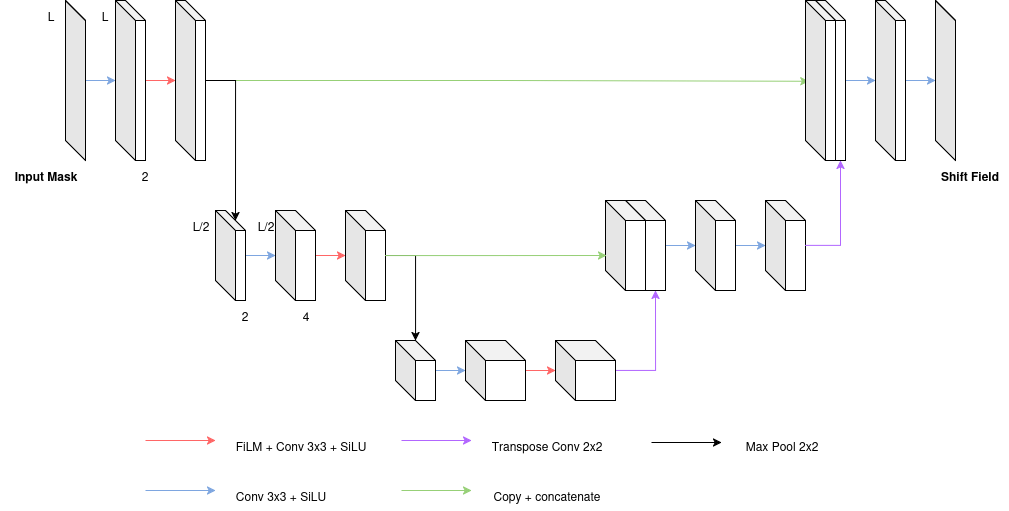
\includegraphics[width=\textwidth]{figures/UNet.png} \\
	\vspace{1cm}
	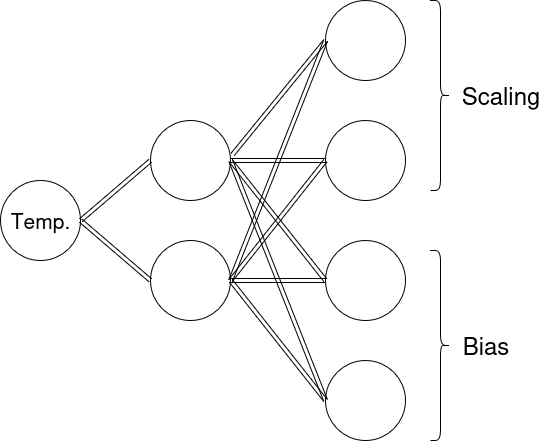
\includegraphics[width=0.4\textwidth]{figures/FiLM.png}
	\end{center}
	\caption{Top: The U-Net architecture we use in this project. Here we only depict the network with 3 levels to the "U", but
	it is easy to extend to an arbitrary number of levels, as long as the length and width of the layer remains integer, of course.
	At each level during the encoder step, a FiLM layer is applied to introduce a dependence on temperature. The final layer
	at each decoder step is saved and appended to the corresponding layer at each decoding step to preserve important long-range
	structure information. The 3rd dimension of each block in the diagram represents the number of channels, and is labeled in the first two
	levels. We double the number of channels at each encoder level, and halve them at each decoder level. \\
	Bottom: The MLP implicit in each FiLM layer. The scalar input is the temperature and the output is two times the number of
	channels at each decoder level. Half of the outputs are used for scaling, the other half for bias.}
	\label{fig:unet}
\end{figure}

As we will ultimately be working with a $128\times128$ lattice, we choose to let the image size at the bottom of the U-Net
be $16\times16$, meaning there will be three FiLM MLPs. In total, there are $7,681$ learnable parameters, around
half of the number of angles on the lattice. 

In order to train the model to generalize to arbitrary temperature and separation, we must improve on the loss function $\ref{eq:loss}$, in which $\mathcal{Q}$
is explicitly a function of $\mathbf{r}$ and implicitly depends on temperature $T$. We write the generalized loss as

\begin{equation}
	\mathcal{L} = \sum_{\mathbf{r}\in\Lambda}g(\mathbf{r})\int_{T_{\min}}^{T_{\max}}\mathrm{d}T\, f(T)\left\langle \left(\mathrm{Re}\,\mathcal{Q}(\mathbf{r})\right)^2 \right\rangle
\end{equation}

where $f$ and $g$ have \textit{support} on the sets $\{\mathbf{r} \,|\, \mathbf{r} \in \Lambda \}$
and $[T_{\min},\,T_{\max}]$ will do. As discussed in \cite{albergo2025netsnonequilibriumtransportsampler}, optimizing loss functions of this type will lead the network 
to individually minimize each contribution to the sum/integral, which is exactly what we hope to achieve --- optimal performance over all separations and temperatures. We opt 
for a particular simple choice of the functions $f$ and $g$, setting them to unity and treating all separations and temperatures on equal footing. If we instead wanting sampling
to be uniform in $\beta=1/T$, we would choose $\rho(T)=\left| d\beta/dT \right|=1/T^2$.

\subsubsection{Training Procedure}

In pratice, we use $4500$ thermalized configurations for temperatures between $0.7$ and $1.1$ in increments of $0.01$, leading to nearly $200,000$ total samples for training of the U-Net.
On top of this, there are $16,384$ possible choices of $\mathbf{r}$ on any one of those lattices.

\section{Implementation}

The entire codebase for this project is available \href{https://github.com/amshak01/XY-Contour-Deformations}{here on GitHub}. In this
section we review the software implementation of the MCMC sampling and deformation of the correlator used. The sampling algorithm
is implemented in C, while the machine learning routines and data post-processing are done in Python files and notebooks.

\subsection{Data Generation and Storage}

\subsection{PyTorch}

\section{Results}

\section{Conclusion}

\begin{appendices}

	\section{KT-Theory}

	\section{FCNs}

	\section{Statistics }

\end{appendices}

\end{document}